\documentclass{article}

\usepackage[english]{babel}
\usepackage{float}
\usepackage[letterpaper,top=2cm,bottom=2cm,left=3cm,right=3cm,marginparwidth=2cm]{geometry}
\usepackage{amsmath}
\usepackage{amssymb}
\usepackage{graphicx}
\usepackage{grffile}
\usepackage{booktabs}
\usepackage{array}
\usepackage{tabularx}
\usepackage{caption}
\usepackage{verbatim}
\usepackage{xcolor}
\usepackage{fancyvrb}
\captionsetup[figure]{justification=centering}
\usepackage[colorlinks=true, allcolors=blue]{hyperref}
\setlength{\emergencystretch}{3em}

\title{\textbf{ME 144L Lab 10: PMDC Motor Speed Control}}
\author{Alejandro Diaz \\ TA: Gabrielle Naquila}
\date{April 28, 2026}

\begin{document}
\maketitle

\tableofcontents
\newpage

% ═══════════════════════════════════════════════════════════════════
\section{Part 1: Open-Loop Speed Control}
% ═══════════════════════════════════════════════════════════════════

% ───────────────────────────────────────────
\subsection{Open-Loop Gain Determination (10\%)}
% ───────────────────────────────────────────

The open-loop (OL) gain $G_{OL}$ [PWM/(rad/s)] relates a desired motor shaft speed directly to the integer PWM command sent to the H-bridge:
\begin{equation}
    \mathrm{PWM}_{cmd} = G_{OL}\,\omega_{m,\mathrm{ref}}
    \label{eq:ol_gain}
\end{equation}

To determine $G_{OL}$ experimentally, the motor was held at constant PWM values from 0 to 255 in increments of 25, and the steady-state shaft speed from the quadrature encoder was recorded in Python via serial communication. Below PWM\,$\approx 55$ the electromagnetic torque was insufficient to overcome Coulomb stiction, so those points were excluded from the regression. A through-origin linear regression (sklearn \texttt{LinearRegression(fit\_intercept=False)}) was applied to the spinning data, yielding:
\begin{equation}
    \boxed{\; G_{OL} = 0.7457~\text{PWM/(rad/s)}, \quad R^2 = 0.9837 \;}
    \label{eq:ol_gain_result}
\end{equation}

Figure~\ref{fig:ol_gain} shows the resulting fit. The high $R^2$ value confirms that a through-origin linear model adequately captures the motor's PWM-to-speed relationship over the spinning range. During the Arduino implementation, the gain is applied as an integer command with saturation:
\begin{equation}
    \mathrm{PWM}_{cmd} = \mathrm{clip}\!\left(\mathrm{round}(G_{OL}\,\omega_{m,\mathrm{ref}}),\ 0,\ 255\right)
    \label{eq:ol_cmd}
\end{equation}

\begin{figure}[H]
    \centering
    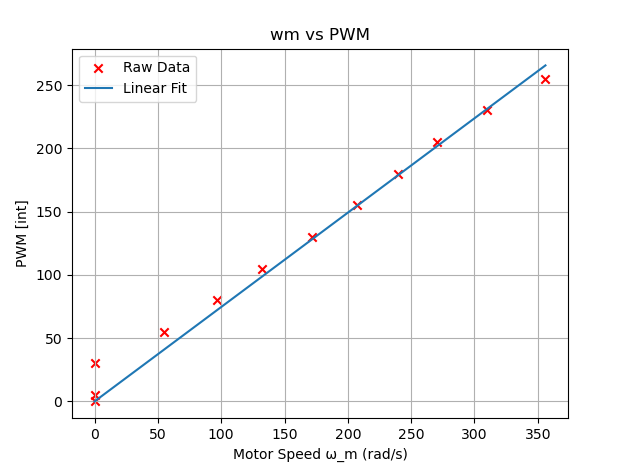
\includegraphics[width=0.78\linewidth]{figures/xlsx_extracted/01_col7_row0.png}
    \caption{OL gain determination: measured PWM vs.\ steady-state motor shaft speed $\omega_m$. A through-origin linear regression on the spinning data points yields $G_{OL} = 0.7457~\text{PWM/(rad/s)}$ with $R^2 = 0.9837$. Points below the stiction threshold are shown but excluded from the fit.}
    \label{fig:ol_gain}
\end{figure}

For closed-loop work, the gain was tuned down to $G_{OL,\text{tuned}} = 0.70~\text{PWM/(rad/s)}$ to reduce the feedforward aggressiveness and give the PID corrective terms more authority.

% ───────────────────────────────────────────
\subsection{Open-Loop Control Performance (15\%)}
% ───────────────────────────────────────────

The OL controller (Eq.~\eqref{eq:ol_gain}) was tested at three reference speeds representative of the motor's operating range. At each setpoint, the Arduino sent the integer-rounded PWM command and the serial monitor logged the reference, measured speed, and error at steady state. Table~\ref{tab:ol_perf} summarizes the results; the error convention is $\Delta\omega = \omega_{m,\mathrm{ref}} - \omega_{m,\mathrm{exp}}$ (negative means the motor ran faster than commanded).

\begin{table}[H]
    \centering
    \caption{Open-loop speed control performance at three reference speeds. $\omega_{m,\mathrm{exp}}$ is the measured steady-state motor shaft speed; $\Delta\omega = \omega_{m,\mathrm{ref}} - \omega_{m,\mathrm{exp}}$ (negative = motor overshoots reference).}
    \label{tab:ol_perf}
    \begin{tabular}{ccccc}
        \toprule
        $\omega_{m,\mathrm{ref}}$ [rad/s] & $\omega_{m,\mathrm{exp}}$ [rad/s] & PWM$_{\mathrm{out}}$ [Int] & $\Delta\omega$ [rad/s] & $|\Delta\omega|$ [\%] \\
        \midrule
        250 & 261.80 & 186 & $-11.80$ & $4.72\%$ \\
        300 & 303.69 & 224 & $-3.69$  & $1.23\%$ \\
        350 & 366.49 & 255 & $-16.49$ & $4.71\%$ \\
        \bottomrule
    \end{tabular}
\end{table}

The motor overshoots the reference at all three setpoints (negative errors). The overshoot is smallest at $\omega_{m,\mathrm{ref}} = 300~\text{rad/s}$ (1.23\%) where the regression captures the operating point most accurately. At $\omega_{m,\mathrm{ref}} = 350~\text{rad/s}$, the required PWM of $0.7457 \times 350 = 260.9$ exceeds the hardware limit of 255, so the motor receives maximum voltage and runs beyond the intended setpoint. The 4.72\% overshoot at 250~rad/s reflects normal scatter about the regression line: the individual data point does not fall exactly on the best-fit line.

Figure~\ref{fig:ol_step} shows the raw time-series for the step test at $\omega_{m,\mathrm{ref}} = 250~\text{rad/s}$. The left subplot shows the motor speed tracking the 250~rad/s reference (with characteristic overshoot), together with the constant PWM command of 186. The right subplot shows the speed error, which settles to approximately $-10~\text{rad/s}$ at steady state. The transient error spike at step onset reflects the encoder lag before the motor reaches speed.

\begin{figure}[H]
    \centering
    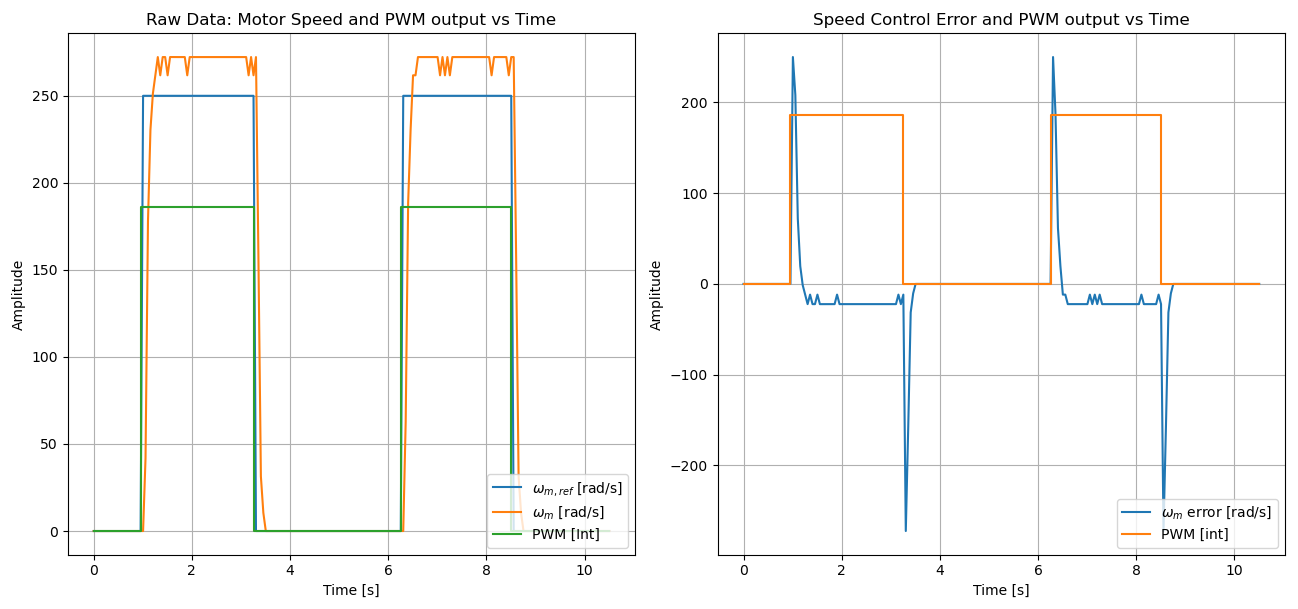
\includegraphics[width=0.92\linewidth]{figures/xlsx_extracted/04_col6_row99.png}
    \caption{Open-loop step test at $\omega_{m,\mathrm{ref}} = 250~\text{rad/s}$ (PWM = 186). Left: measured motor speed (orange) and reference (blue) with PWM output (green). Right: speed error and PWM vs.\ time. The motor consistently overshoots the reference, producing a steady-state error of approximately $-10~\text{rad/s}$.}
    \label{fig:ol_step}
\end{figure}

% ───────────────────────────────────────────
\subsection{Open-Loop Stability Discussion (5\%)}
% ───────────────────────────────────────────

Open-loop control cannot become unstable in the feedback sense because there is no signal path from the plant output back to the controller input. Instability in a closed-loop system requires a loop gain and phase condition (Nyquist / Bode criterion) that simply does not exist when the controller and plant are not connected in a loop. For the PMDC motor, the equation of motion
\begin{equation}
    J_m\,\dot{\omega}_m = r_m\,i_m - B_m\,\omega_m - \tau_{mo}\,\tanh(\omega_m)
    \label{eq:eom}
\end{equation}
with $i_m = (V_{in} - r_m\,\omega_m)/R_m$ is an inherently stable first-order plant: for any bounded constant $V_{in}$ the speed converges to a finite equilibrium because viscous and Coulomb friction provide positive damping ($\partial\dot{\omega}_m/\partial\omega_m < 0$). Bounded-input bounded-output (BIBO) stability is therefore guaranteed as long as the commanded voltage stays within the hardware limits, which the PWM clipping to $[0, 255]$ ensures.

The practical limitations of open-loop control are not stability but accuracy. Because the gain $G_{OL}$ is a single empirically derived constant, it cannot compensate for:
\begin{itemize}
    \item \textbf{PWM saturation}: at $\omega_{m,\mathrm{ref}} = 350~\text{rad/s}$ the required command exceeds 255, the motor receives full voltage, and the speed cannot be regulated.
    \item \textbf{Load and voltage disturbances}: any change in supply voltage $V_b$, motor temperature, or external load torque shifts the steady-state speed without the controller reacting, producing a persistent error that cannot self-correct.
    \item \textbf{Regression scatter}: individual operating points deviate from the best-fit line (as shown in Table~\ref{tab:ol_perf}), so the OL gain cannot eliminate steady-state error at every setpoint simultaneously.
\end{itemize}

These are the motivating limitations that make closed-loop feedback control advantageous.

% ───────────────────────────────────────────
\subsection{Open-Loop Performance with Added Load Inertia (25\%)}
% ───────────────────────────────────────────

\subsubsection*{Inertia calculation}

A solid aluminum disk (mass $m_d = 390~\text{g}$, radius $r_d = 101.5~\text{mm}$) was mounted on the \emph{output} shaft of the gearbox. The disk's rotational inertia about its spin axis is:
\begin{equation}
    J_{\text{disk}} = \tfrac{1}{2}\,m_d\,r_d^2
    = \tfrac{1}{2}(0.390)(0.1015)^2
    = 2.009 \times 10^{-3}~\text{kg}\!\cdot\!\text{m}^2
\end{equation}

Because the disk spins at the output-shaft speed ($\omega_{\text{out}} = \omega_m / GR$), its inertia reflected to the motor shaft through the gearbox ratio $GR = 45$ is:
\begin{equation}
    J_{\text{refl}} = \frac{J_{\text{disk}}}{GR^2}
    = \frac{2.009 \times 10^{-3}}{45^2}
    = 9.92 \times 10^{-7}~\text{kg}\!\cdot\!\text{m}^2
    \label{eq:j_refl}
\end{equation}

The total effective motor-shaft inertia becomes:
\begin{equation}
    J_{\text{eff}} = J_m + J_{\text{refl}}
    = 1.45 \times 10^{-7} + 9.92 \times 10^{-7}
    = 1.137 \times 10^{-6}~\text{kg}\!\cdot\!\text{m}^2
    \approx 7.8\,J_m
    \label{eq:j_eff}
\end{equation}

\subsubsection*{Effect on open-loop step response}

Inertia governs the transient dynamics through the mechanical time constant $\tau_m = J_m / (r_m^2/R_m + B_m)$. With the disk, $\tau_m$ increases by a factor of $J_{\text{eff}}/J_m = 7.8$, so the motor takes approximately 7.8 times longer to reach steady-state speed after a step change. The steady-state speed itself is unchanged because it depends only on the torque balance at equilibrium---$r_m$, $R_m$, $B_m$, $\tau_{mo}$, and $V_{in}$ are all unaffected by the disk.

\noindent\textit{Note:} The inertia step test was conducted with the tuned feedforward gain $G_{OL,\text{tuned}} = 0.70~\text{PWM/(rad/s)}$ (giving PWM $= 175$ at $\omega_{ref} = 250~\text{rad/s}$), not the original regression gain $G_{OL} = 0.7457$ used in Section~1.2 (which gave PWM $= 186$). The transient comparison is therefore at a slightly different operating point, though the qualitative conclusion---that the 7.8$\times$ inertia increase dramatically slows the rise---is unaffected.

Figure~\ref{fig:ol_inertia} shows the OL step test at $\omega_{m,\mathrm{ref}} = 250~\text{rad/s}$ after the disk was mounted. Comparing the left subplot (motor speed vs.\ time) against Figure~\ref{fig:ol_step}: without the disk the motor reaches steady state in under 0.5~s; with the disk the speed rises slowly and the reference window ends before the motor fully settles. The right subplot confirms a large persistent speed error ($\approx +25~\text{rad/s}$, positive meaning the motor is still \emph{below} the reference) during the step-on period, followed by a symmetric undershoot when the reference returns to zero.

\begin{figure}[H]
    \centering
    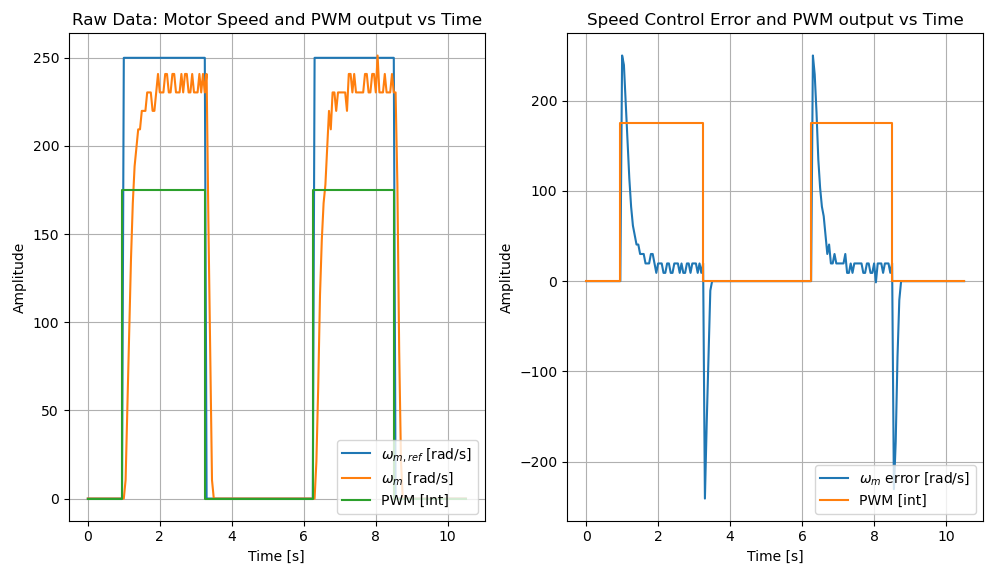
\includegraphics[width=0.92\linewidth]{figures/xlsx_extracted/06_col7_row133.png}
    \caption{Open-loop step test at $\omega_{m,\mathrm{ref}} = 250~\text{rad/s}$ with the inertia disk mounted on the output shaft ($J_{\text{eff}} = 1.14 \times 10^{-6}~\text{kg}\!\cdot\!\text{m}^2$, $7.8 \times J_m$). The motor cannot reach the reference within the commanded window, and the error plot confirms that the 7.8$\times$ increase in effective inertia significantly slows the transient without changing the eventual steady-state speed.}
    \label{fig:ol_inertia}
\end{figure}

The implication for open-loop speed control is that high inertia loads degrade tracking for time-varying references. With no feedback to compensate for the slower dynamics, the motor may still be accelerating when the reference changes, causing large positional or velocity errors during maneuvers. Closed-loop control, which continuously corrects the error, is significantly more robust to load inertia changes.

% ═══════════════════════════════════════════════════════════════════
\section{Part 2: Closed-Loop Speed Control}
% ═══════════════════════════════════════════════════════════════════

% ───────────────────────────────────────────
\subsection{PID + Feedforward Tuned Results (15\%)}
% ───────────────────────────────────────────

The closed-loop speed controller combines a feedforward (FF) term based on the tuned OL gain and a discrete PID feedback term. In the Arduino implementation (from \texttt{PMDC\_CL\_Control\_DAQ.ino}), the total PWM command at each loop iteration $k$ is:
\begin{equation}
    \mathrm{PWM}_k = G_{FF}\,\omega_{ref} + K_p\,e_k + K_i\!\sum_{j=0}^{k} e_j\,\Delta t_j + K_d\,\frac{e_k - e_{k-1}}{\Delta t_k}
    \label{eq:pid_ff}
\end{equation}
where $e_k = \omega_{m,\mathrm{ref}} - \omega_{m,k}$ is the speed error, $\Delta t_k$ is the loop sample period in seconds, and $G_{FF} = 0.70~\text{PWM/(rad/s)}$ is the tuned feedforward gain. The final tuned closed-loop gains are:
\begin{equation}
    \boxed{K_p = 0.05~\frac{\text{PWM}}{\text{rad/s}}, \quad
           K_i = 0.10~\frac{\text{PWM}}{\text{rad}}, \quad
           K_d = 0.0}
    \label{eq:cl_gains}
\end{equation}

Figure~\ref{fig:cl_pid_ff} shows the tuned CL step response with reference speed alternating between 300 and 200~rad/s. The motor tracks both setpoints with fast rise times and errors that settle to near zero within 1--2 seconds of each step change. The integral term eliminates the persistent steady-state overshoot that characterized the open-loop results.

\begin{figure}[H]
    \centering
    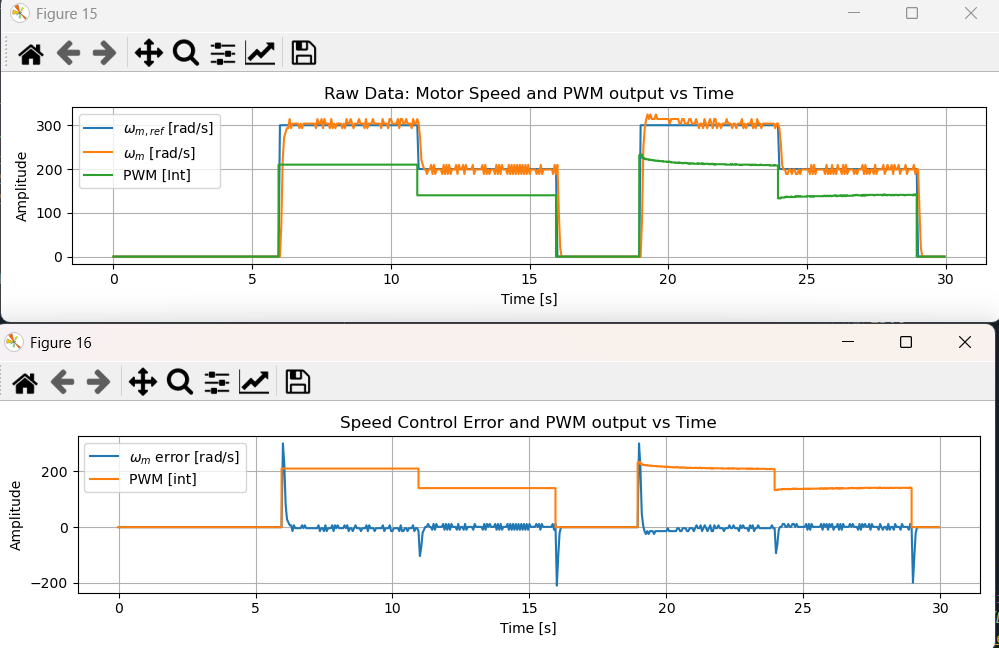
\includegraphics[width=0.94\linewidth]{figures/xlsx_extracted/10_col7_row205.png}
    \caption{Closed-loop PID+FF step test (no inertia disk). The motor alternates between $\omega_{ref} = 300~\text{rad/s}$ and $200~\text{rad/s}$ over approximately 30 seconds. Top (Figure~15): motor speed (orange) closely tracks the reference (blue) with PWM output (green) adjusting in real time. Bottom (Figure~16): speed error decays to within a few rad/s of zero at steady state. Tuned gains: $G_{FF} = 0.70$, $K_p = 0.05$, $K_i = 0.10$, $K_d = 0$.}
    \label{fig:cl_pid_ff}
\end{figure}

% ───────────────────────────────────────────
\subsection{PID Gain Selection Process (10\%)}
% ───────────────────────────────────────────

Gain tuning followed a sequential approach, starting from the feedforward baseline and adding corrective terms one at a time.

\textbf{Step 1: Feedforward gain.} The feedforward gain was reduced from the original regression value (0.7457) to $G_{FF} = 0.70~\text{PWM/(rad/s)}$. This deliberate under-command gives the proportional and integral terms room to correct upward, avoiding the integrator windup that results when the FF alone overshoots the reference and the integral drives the PWM below the FF value.

\textbf{Step 2: Proportional gain $K_p$.} With $G_{FF} = 0.70$ and $K_i = K_d = 0$, the controller was a pure proportional+FF loop. $K_p$ was set to $0.05~\text{PWM/(rad/s)}$, chosen because larger values ($K_p \geq 0.10$) produced noticeable overshoot and oscillation at step transitions due to the encoder noise amplifying the derivative-like response of a fast proportional gain.

\textbf{Step 3: Integral gain $K_i$.} With $K_p = 0.05$ a small residual steady-state offset remained (motor running 5--10~rad/s below reference due to the deliberately reduced FF). Setting $K_i = 0.10~\text{PWM/(rad/s)}$ eliminated the offset; the integral term accumulated enough command over 1--2 seconds to fully bridge the FF gap. Higher values of $K_i$ were found to induce integrator windup during the initial startup transient, producing overshoot.

\textbf{Step 4: Derivative gain $K_d$.} A derivative term amplifies encoder noise. Because the speed signal from the 12-CPR encoder at the Arduino's 20~Hz control rate already exhibited $\pm 5~\text{rad/s}$ noise, adding any nonzero $K_d$ caused rapid PWM chattering without a meaningful reduction in overshoot. The derivative gain was therefore set to $K_d = 0$.

The final values in Eq.~\eqref{eq:cl_gains} were validated at both reference speeds and confirmed to maintain zero steady-state error without oscillation or PWM chattering.

% ───────────────────────────────────────────
\subsection{Effect of Increased Load Inertia on Closed-Loop Control (10\%)}
% ───────────────────────────────────────────

The inertia disk from Section~1.4 ($J_{\text{eff}} = 1.137 \times 10^{-6}~\text{kg}\!\cdot\!\text{m}^2$, $7.8 \times J_m$) was re-mounted and the same CL gains (Eq.~\eqref{eq:cl_gains}) were applied without modification.

Figure~\ref{fig:cl_inertia} shows the loaded step response at the same 300/200~rad/s reference schedule. Comparing Figure~\ref{fig:cl_pid_ff} (unloaded) and Figure~\ref{fig:cl_inertia} (loaded):

\begin{itemize}
    \item \textbf{Steady-state accuracy is preserved.} The integral term drives the error to near zero at both setpoints in both cases because the integrating action is independent of inertia at steady state.
    \item \textbf{The step-up rise is noticeably slower with the disk.} At $t \approx 19~\text{s}$ (second step to 300~rad/s), the motor's rise time is visibly longer in Figure~\ref{fig:cl_inertia} than at $t \approx 6~\text{s}$ in Figure~\ref{fig:cl_pid_ff}, reflecting the 7.8$\times$ inertia increase requiring more time to accelerate.
    \item \textbf{The PWM command is higher during acceleration.} The PWM output in Figure~\ref{fig:cl_inertia} reaches approximately 225 during the step-up phase, compared to 205 in the unloaded case, as the controller works harder against the greater inertia.
\end{itemize}

The key advantage demonstrated here is that closed-loop control \emph{automatically adapts} to the higher inertia: the same gain set still achieves zero steady-state error without any manual retuning, whereas the open-loop controller in Section~1.4 was unable to compensate at all.

\begin{figure}[H]
    \centering
    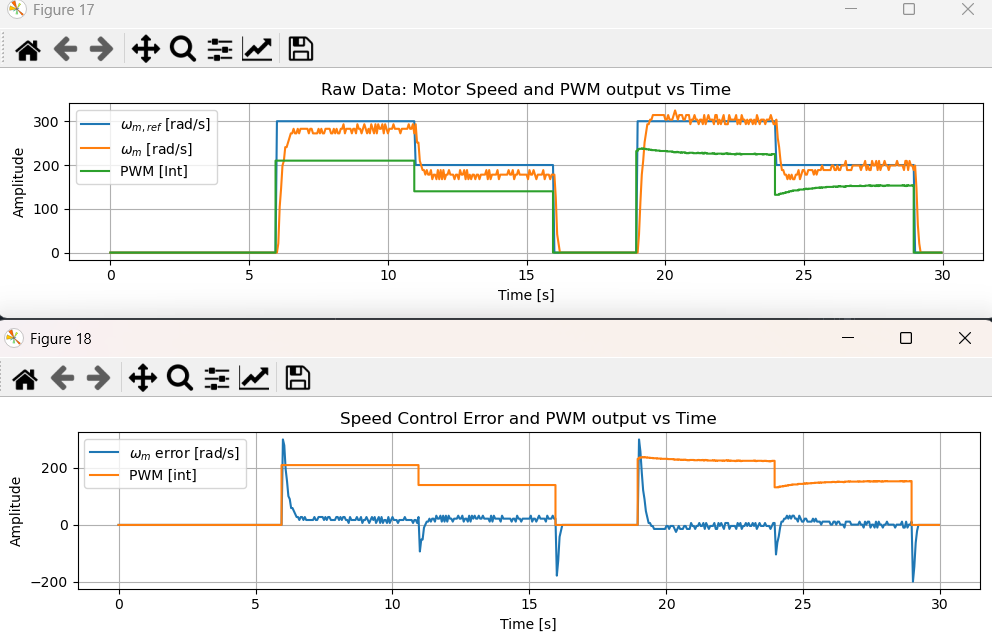
\includegraphics[width=0.94\linewidth]{figures/xlsx_extracted/12_col7_row224.png}
    \caption{Closed-loop PID+FF step test with the inertia disk mounted ($J_{\text{eff}} = 1.14 \times 10^{-6}~\text{kg}\!\cdot\!\text{m}^2$). The same gain set as Figure~\ref{fig:cl_pid_ff} is used. Top (Figure~17): motor speed tracks the 300/200~rad/s reference with a longer rise time than the unloaded case. Bottom (Figure~18): speed error still decays to near zero, confirming the integral action compensates for the added load.}
    \label{fig:cl_inertia}
\end{figure}

% ───────────────────────────────────────────
\subsection{Simulation vs.\ Experiment Comparison (10\%)}
% ───────────────────────────────────────────

Two simulation comparisons are presented: one for open-loop steady-state prediction, and one for the full closed-loop transient.

\subsubsection*{OL steady-state: simulation vs.\ experiment}

For each of the three OL setpoints, the physics-based PMDC ODE model (inductance neglected) was integrated to steady state using the commanded voltage $V_{in} = (\mathrm{clip}(G_{OL}\,\omega_{ref}, 0, 255)/255)\,V_b$ with the Lab~9 motor parameters. Figure~\ref{fig:ol_sim_vs_exp} compares the simulated and measured steady-state speeds.

\begin{figure}[H]
    \centering
    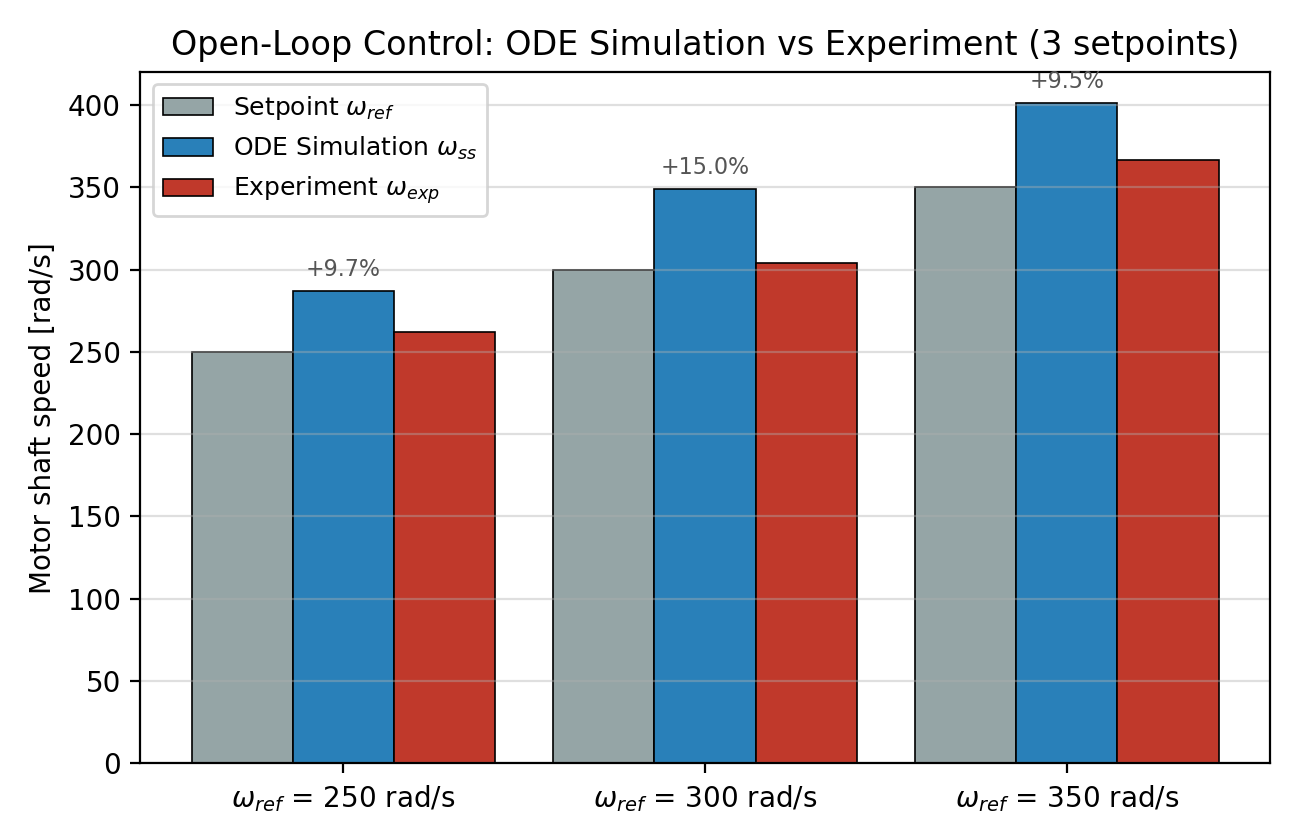
\includegraphics[width=0.78\linewidth]{figures/ol_sim_vs_exp.png}
    \caption{Grouped bar chart comparing the ODE model steady-state prediction vs.\ experimental measurement at three OL setpoints. The annotated percentages are the errors $({\omega_{sim}-\omega_{exp}})/{\omega_{exp}}$. The model consistently over-predicts speed by 9--15\% because the Lab~9 friction characterization underestimates losses at these mid-range operating points.}
    \label{fig:ol_sim_vs_exp}
\end{figure}

The ODE model over-predicts motor speed by 9.7\% at 250~rad/s, 15.0\% at 300~rad/s, and 9.5\% at 350~rad/s. This systematic positive bias means the friction model ($B_m = 4.71 \times 10^{-7}~\text{N}\!\cdot\!\text{m}\!\cdot\!\text{s/rad}$, $\tau_{mo} = 9.81 \times 10^{-5}~\text{N}\!\cdot\!\text{m}$) underestimates the real dissipation at these operating points. The empirical OL gain regression, by contrast, captures the aggregate real-motor behavior directly and so maps 0.7457$\,\omega_{ref}$ to the correct steady-state speed more accurately.

\subsubsection*{CL transient: simulation vs.\ experiment}

The same ODE motor model was connected to the discrete PID+FF controller (Eq.~\eqref{eq:pid_ff}, $G_{FF}=0.70$, $K_p=0.05$, $K_i=0.10$, $K_d=0$) at a 20~Hz sample rate and simulated over the same 300/200~rad/s reference schedule as the experiment. Figure~\ref{fig:cl_sim} shows the result.

\begin{figure}[H]
    \centering
    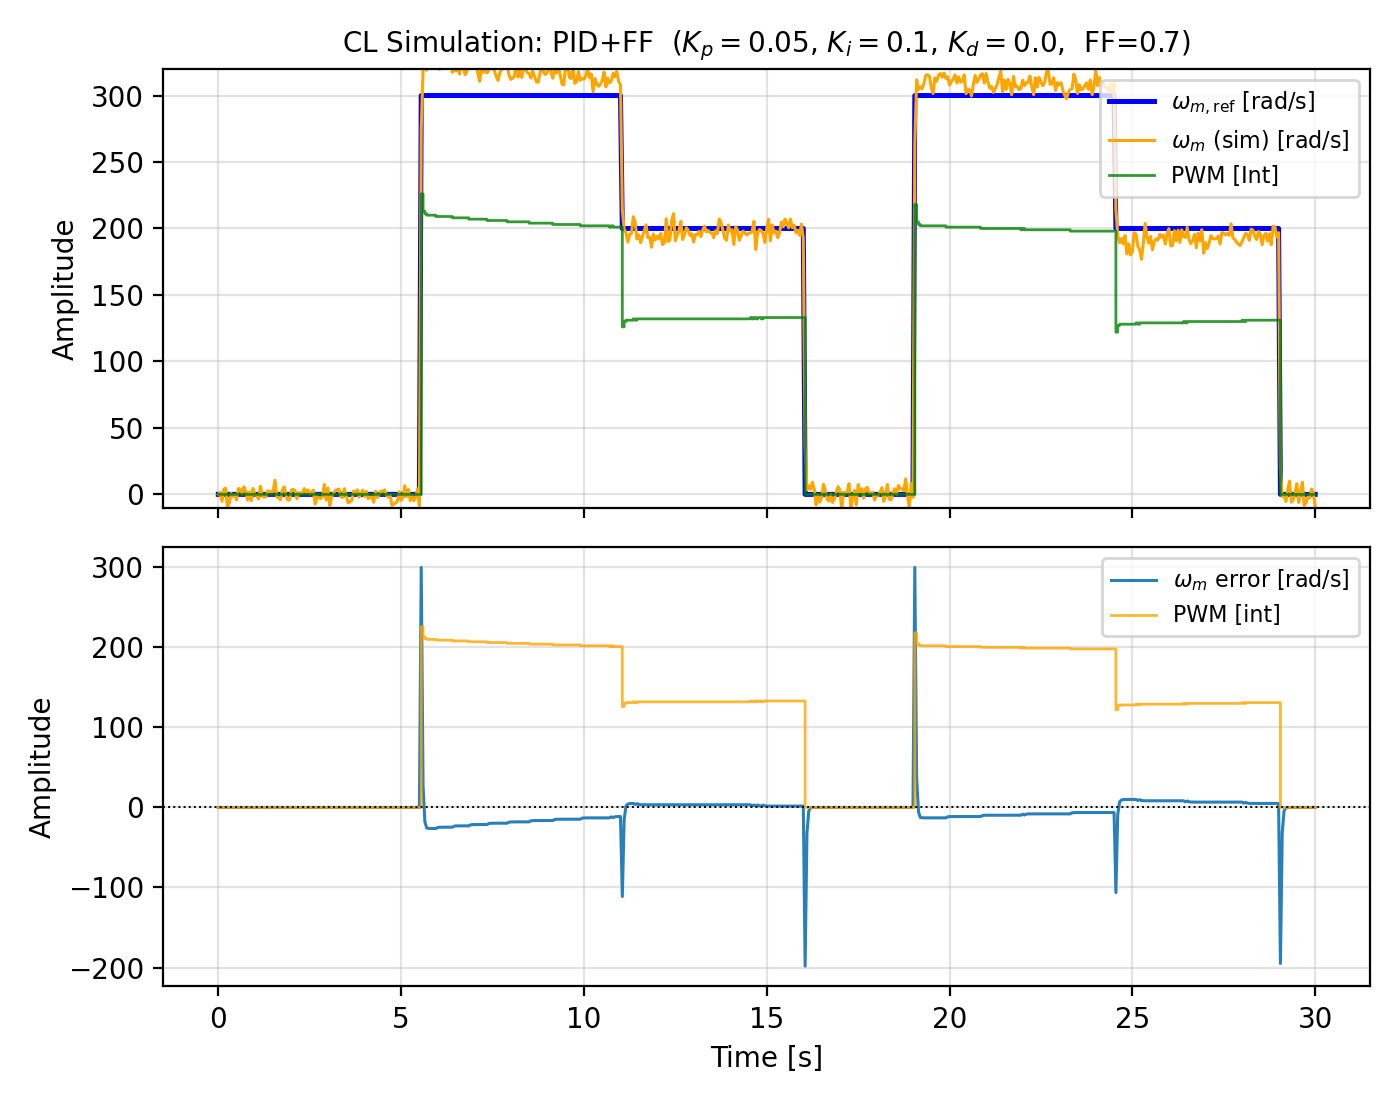
\includegraphics[width=0.88\linewidth]{figures/cl_sim_step.png}
    \caption{Closed-loop PID+FF simulation (same reference schedule as Figure~\ref{fig:cl_pid_ff}). Top: simulated motor speed (orange) tracks the 300/200~rad/s reference (blue), with PWM output (green). Bottom: speed error and PWM. The simulation shows qualitatively similar fast tracking with integral-eliminated steady-state error, but the ODE model over-predicts the steady-state speed by $\sim$5\% relative to the reference due to the same friction-model mismatch identified in Figure~\ref{fig:ol_sim_vs_exp}.}
    \label{fig:cl_sim}
\end{figure}

\subsubsection*{Qualitative assessment}

Both simulation and experiment show:
\begin{enumerate}
    \item Fast step response ($< 1.5~\text{s}$ rise time to first setpoint).
    \item Integral action driving the steady-state error to near zero.
    \item PWM adjusting dynamically at each step change, not saturating.
    \item Smooth tracking without oscillation.
\end{enumerate}

The main quantitative discrepancy is that the simulation's steady-state speed converges to approximately 315~rad/s when the reference is 300~rad/s, reflecting the same over-prediction bias seen in the OL comparison. The integral term partially compensates, but because the ODE model itself predicts a higher speed for a given voltage, the integrator must reduce the PWM below the FF command to hold the modeled speed at the reference. In the real motor the friction losses are higher, so the actual motor settles closer to the reference with less integral correction required.

\subsubsection*{Sources of discrepancy and improvements}

The primary source of error is the Lab~9 friction model. Refining $\tau_{mo}$ by fitting low-speed (60--120~rad/s) data points separately, where Coulomb friction dominates, would reduce the over-prediction. A secondary improvement would be to include a static-friction (stiction) term that prevents motion below a threshold torque, capturing the PWM dead-zone observed experimentally. Finally, validating the motor inertia $J_m$ independently (e.g., via the log-decrement method from the Lab~9 coastdown trace) would reduce uncertainty in the transient time constant.

\end{document}
